\section{Le circuit logique} \label{sec:logique}
%%%%%%%%%%%%%%%%%%%%%%%%%%%%%%%%%%%%%%%%%%%%%%%%%%%%%%%%%%%%%%%%%%%
%%%%%%%%%%%%%%%%%%%%%%%%%%%%%%%%%%%%%%%%%%%%%%%%%%%%%%%%%%%%%%%%%%%
Le niveau plus bas abordé dans cette thèse est celui des transistors qui sont les composants de bases de tout système électronique. 

\subsection{Les Transistors}
%%%%%%%%%%%%%%%%%%%%%%%%%%%%%%%%%%%%%%%%%%%%%%%%%%%%%%%%%%%%%%%%%%%
Le premier transistor a été mis au point par des chercheurs des Laboratoires Bell en 1947 \cite{bardeen1948transistor} dont la découverte avait été réalisée quelque années avant \cite{edgar1930method}. Ils apparaissent comme une révolution face aux tubes électroniques utilisés jusque là (plus rapide, léger et robuste). Un transistor est un composant électronique qui utilise trois bornes: la base, l’émetteur et le collecteur (voir \autoref{pic:transistor}). Le collecteur est relié au fil d’où vient la tension et correspond à la sortie du transistor. L’émetteur est lui relié à la masse (tension 0 volt). La base constitue la connexion en connecteur et émetteur en fonction de la tension qui lui est appliquée. En appliquant une tension faible à la base, le courant entre le collecteur et l’émetteur est possible. Sans aucune tension appliquée à la base, le passage du courant n’est pas possible. Pour les personnes non familières avec ces concepts électriques, une approche vulgarisée peut être utilisée \cite{JohnLeDuc2017}. Ainsi, le transistor se comporte comme un interrupteur binaire très rapide (basculement en quelques nanosecondes $10^{-9}$ seconde).



\begin{figure}[htbp]
    \centering
    \begin{subfigure}[b]{0.45\linewidth}\centering
        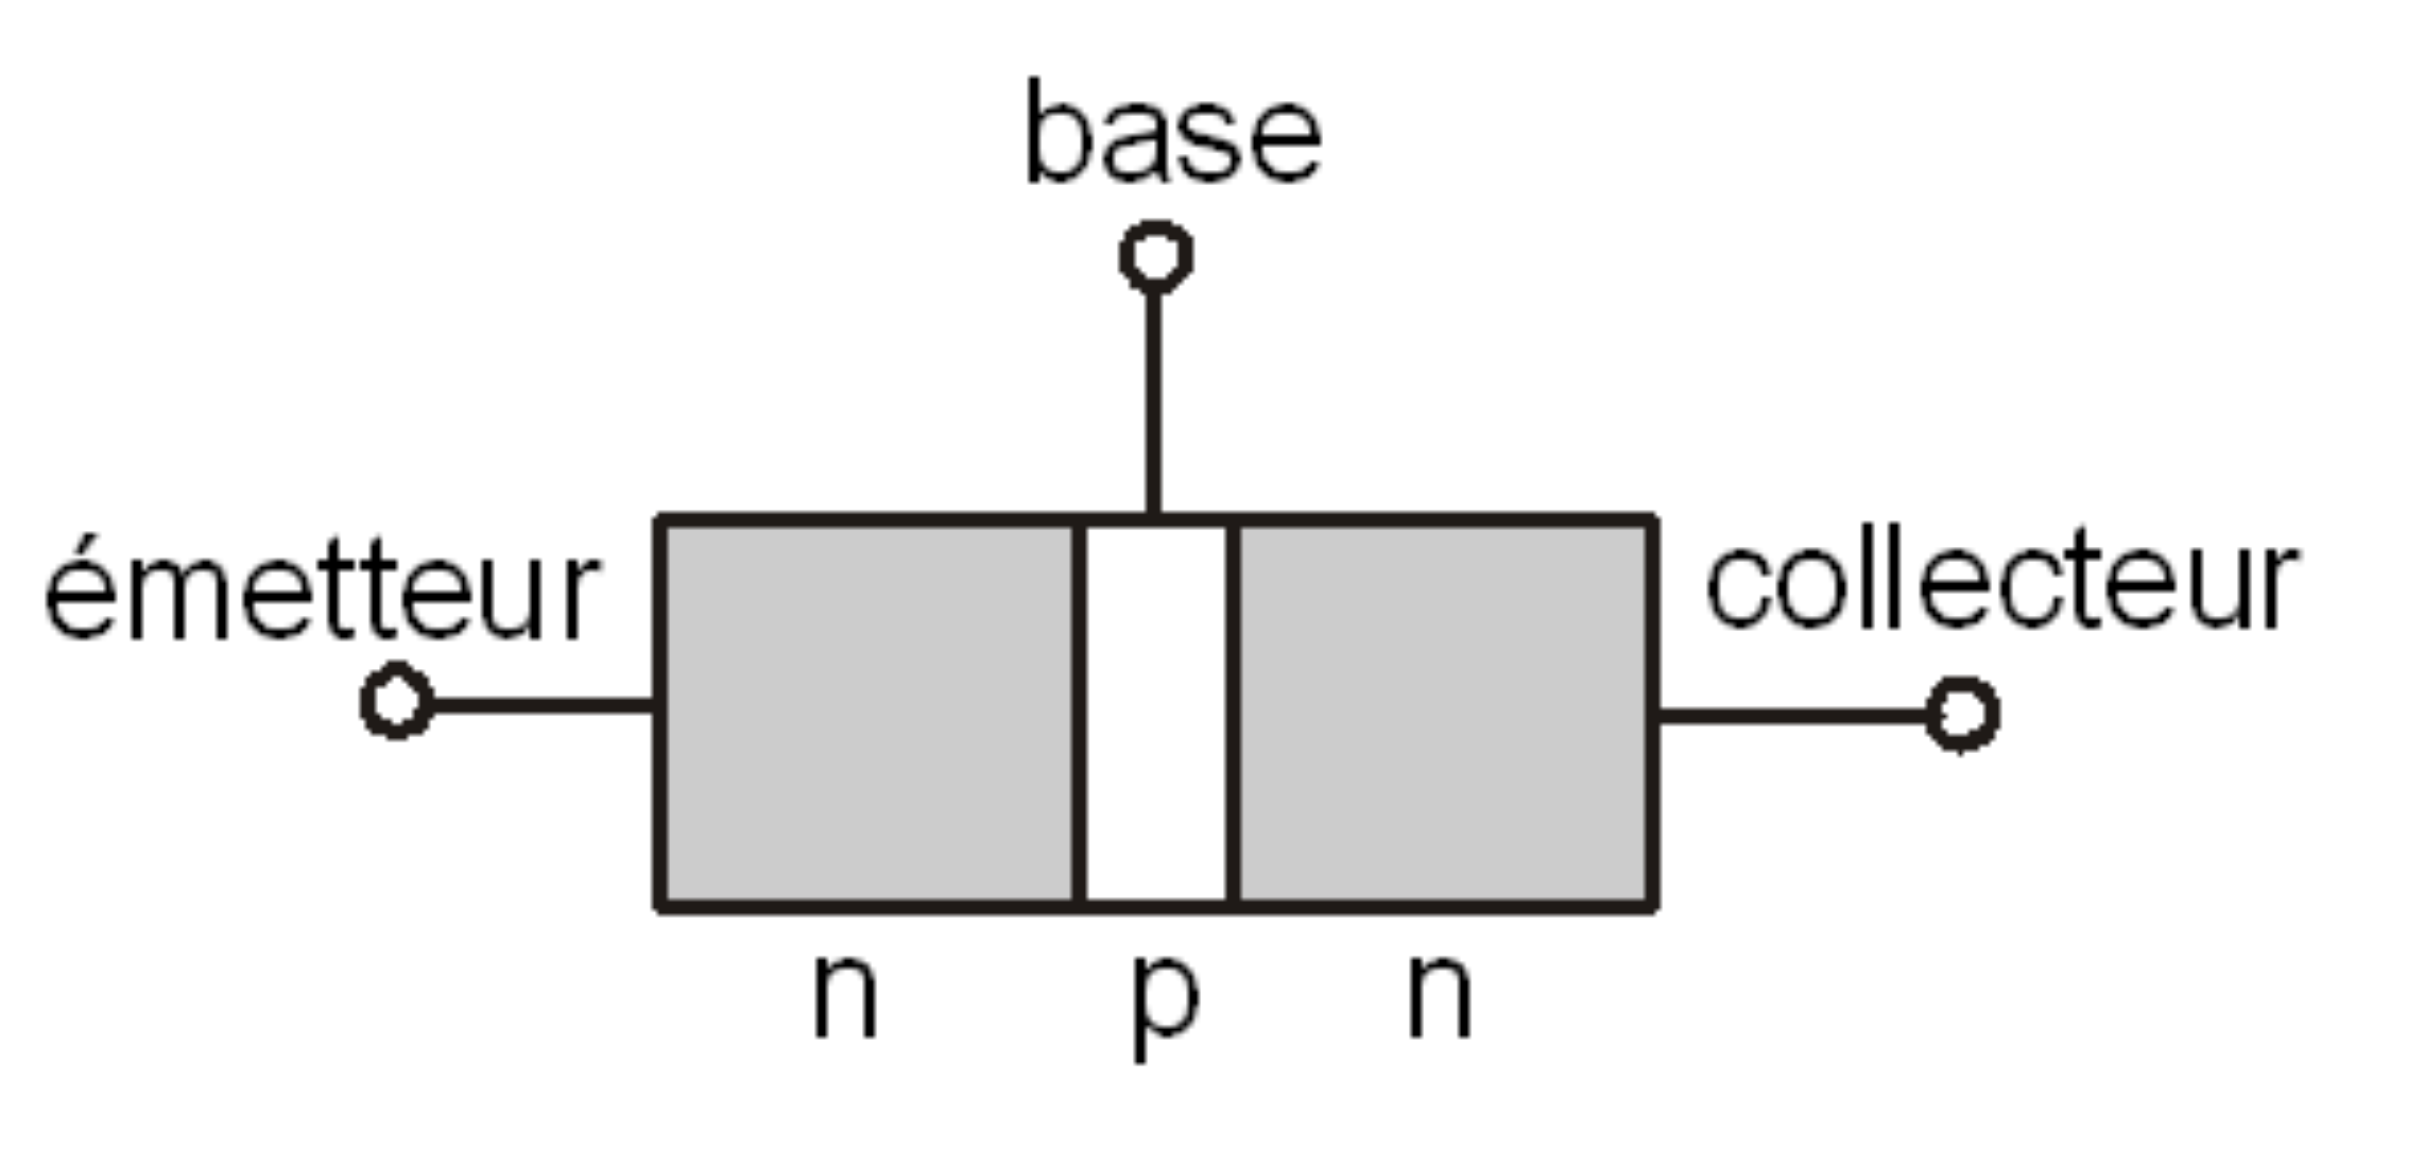
\includegraphics[width=\linewidth]{images/transistor.png}
        \caption{\label{pic:transistor} Schéma d'un transistor NPN \cite{GeraldHuguenin2018}}.
    \end{subfigure}
    ~ %add desired spacing between images, e. g. ~, \quad, \qquad, \hfill etc.
      %(or a blank line to force the subfigure onto a new line)
    \begin{subfigure}[b]{0.45\linewidth}\centering
        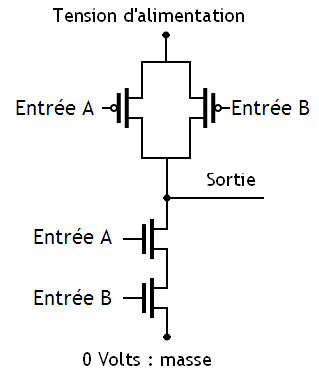
\includegraphics[width=0.5\linewidth]{images/processeur_porte_nand.png}
        \caption{\label{pic:processeur_porte_nand} Schéma électrique d'une porte \textit{NON-ET} réalisée à partir de 4 transistors \cite{Wikibooks2019PorteNand}}
    \end{subfigure}
    \caption{Un transistor est utilisé pour réaliser des portes complexes  }\label{pic:transistor_usage}
\end{figure}




\subsection{Les portes logiques}
%%%%%%%%%%%%%%%%%%%%%%%%%%%%%%%%%%%%%%%%%%%%%%%%%%%%%%%%%%%%%%%%%%%
Les portes logiques sont construites à partir de transistors et permettent l'exécution de différentes instructions ou la capacité de stocker une information (registres). Par exemple, en associant deux transistors inverseur en série on construit une porte NON-ET qui ne laisse passer le courant seulement lorsqu'aucune ou une des deux entrées a une tension (voir \autoref{pic:processeur_porte_nand})



Une porte logique possède plusieurs entrées numériques qui peuvent être le résultat d'autres portes logiques (voir \autoref{pic:processeur_portes}). Les circuits les plus complexes sont en fait une cascade de milliers de portes logiques comme celles-ci. Il est aussi nécessaire de choisir la signification du passage ou non du courant et construire des portes ayant un « sens ». Il est courant d’utiliser les termes VRAI ou \textit{1 logique} lorsque le courant circule et FAUX ou \textit{0 logique} pour l’absence de tension.


\begin{figure}
\begin{subfigure}{.3\textwidth}
\centering
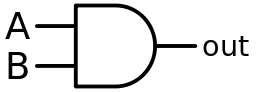
\includegraphics[width=3cm]{images/processeur_porte_et.png}
\caption{La porte \textit{ET} ne laisse passer le courant seulement si les deux entrées sont vraies}
\end{subfigure}\hfill
\begin{subfigure}{.3\textwidth}
\centering
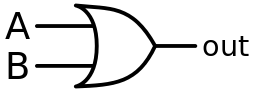
\includegraphics[width=3cm]{images/processeur_porte_ou.png}
\caption{La porte \textit{ET} laisse passer le courant si au moins une des deux entrées est vraies}
\end{subfigure}\hfill
\begin{subfigure}{.3\textwidth}
\centering
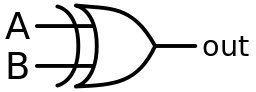
\includegraphics[width=3cm]{images/processeur_porte_oux.png}
\caption{La porte \textit{OU EXCLUSIF} est vrai seulement si les deux entrées ont des valeurs distinctes}
\end{subfigure}
\caption{Représentation graphique de trois portes logiques \cite{Wikipedia2019Porte}}
\label{pic:processeur_portes}
\end{figure}




\subsection{Algèbre de Boole}
%%%%%%%%%%%%%%%%%%%%%%%%%%%%%%%%%%%%%%%%%%%%%%%%%%%%%%%%%%%%%%%%%%%
Analyser le fonctionnement de plusieurs portes peut rapidement se complexifier et le recours à des méthodes algébriques est nécessaire. Les portes pouvant avoir des valeurs de 0 ou 1, un nouveau type d'algèbre a été créée: l'algèbre de Boole. Comme pour l'algèbre en base décimale, l'algèbre booléenne utilise des fonctions et des variables pour décrire le comportement d'un système. Les variables utilisées ne peuvent prendre que deux valeurs. Une table de vérité de fonctions générales peut alors être écrite. On peut écrire une table de vérité d'un programme souhaité, qui utilise trois entrées, et déterminer les sorties ($M$) souhaitées (voir \autoref{pic:processeur_porte_table}). Grâce à l'algèbre de Boole, on peut convertir cette table en circuit implémentant ce fonctionnement (\autoref{pic:processeur_porte_schema}).
L'algèbre de Boole est aussi utilisée pour réduire la complexité d'un circuit sans en changer le comportement, notamment grâce à la fameuse loi de DeMorgan \cite{hurley2014concise} permettant le changement de portes \textit{ET} en portes \textit{OU}. En réduisant la complexité et le nombre de portes, il est possible de réaliser des circuits plus économiques et plus rapides.


\begin{figure}[htbp]
    \centering
    \begin{subfigure}[b]{0.40\linewidth}\centering
        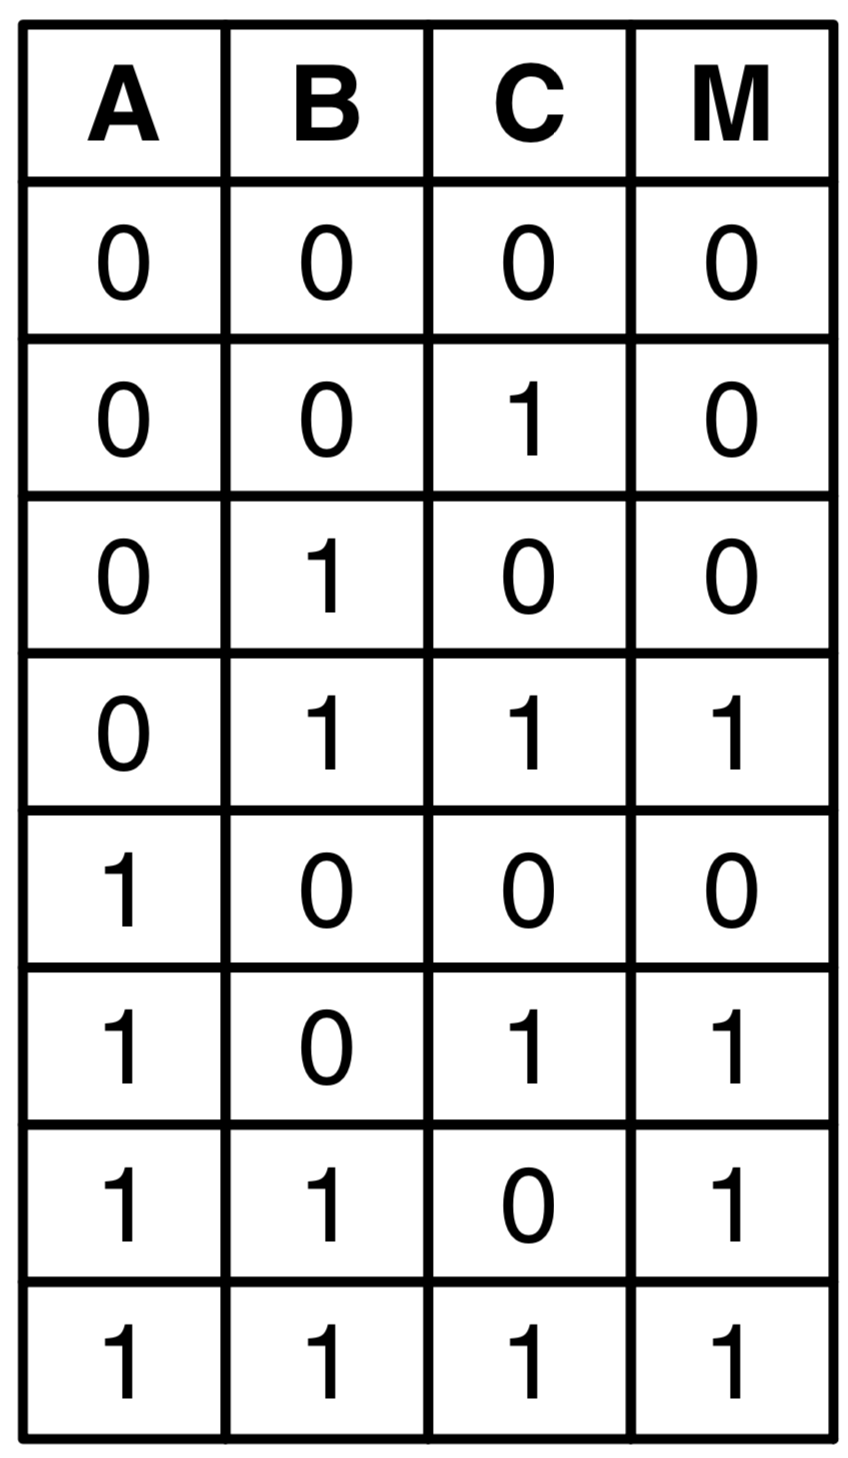
\includegraphics[width=0.4\linewidth]{images/processeur_porte_table.png}
        \caption{Table de vérité d'un circuit souhaité
        \label{pic:processeur_porte_table}}
    \end{subfigure}
    ~ %add desired spacing between images, e. g. ~, \quad, \qquad, \hfill etc.
      %(or a blank line to force the subfigure onto a new line)
    \begin{subfigure}[b]{0.40\linewidth}\centering
        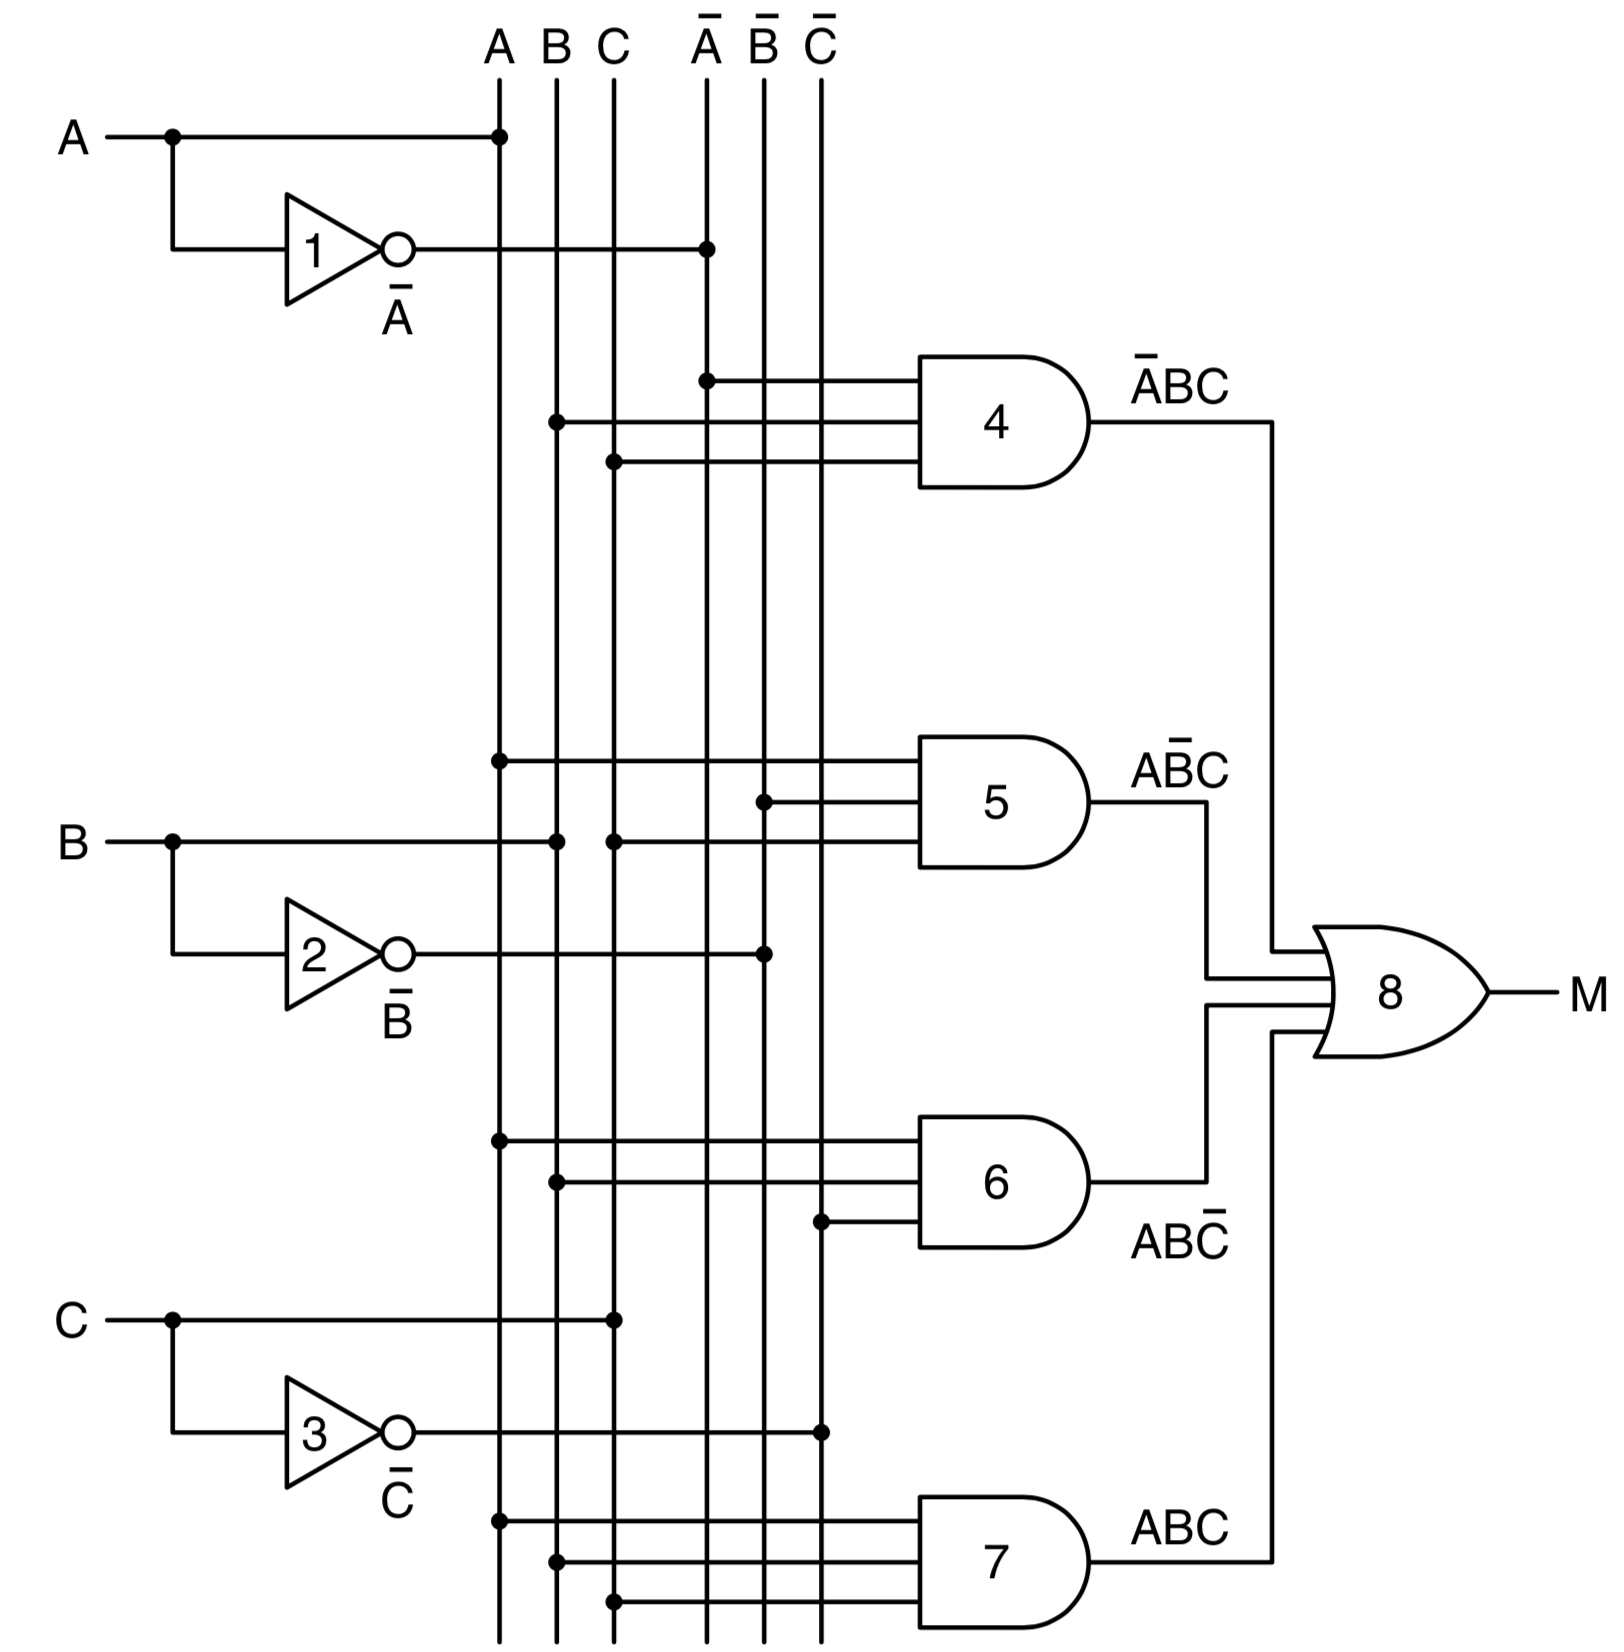
\includegraphics[width=\linewidth]{images/processeur_porte_schema.png}
        \caption{Circuit logiques  utilisant 8 portes
        \label{pic:processeur_porte_schema}}
    \end{subfigure}
    \caption{A partir d'une table de vérité, on peut générer le circuit logique correspondant \cite{tanenbaum2016structured}  \label{pic:processeur_porte_schema}}
\end{figure}




\subsection{Circuits logiques}
%%%%%%%%%%%%%%%%%%%%%%%%%%%%%%%%%%%%%%%%%%%%%%%%%%%%%%%%%%%%%%%%%%%
À partir des portes logiques et de leur analyse avec l'algèbre de Boole des circuits plus complexes peuvent être élaborés qui peuvent être regroupés en deux grandes familles: les circuits logiques de base  et les circuits logiques à mémoire. La principale différence entre les deux vient de leur capacité à retenir une information. 

\subsubsection{Les circuits logiques de base}
Les circuits logiques de base contiennent les circuits intégrés qui sont des circuits pouvant comporter quelques centaines de portes (circuit SSI, MSI) ou plusieurs centaines de milliers (circuit LSI et VLSI) \cite{barbe2013very}.
Les circuits combinatoires ne dépendent que des entrées ne possédant pas de mémoire interne pouvant influer sur le résultat. Parmi eux, nous pouvons citer le multiplexeur (qui permets de choisir une entrée parmi plusieurs), les circuits arithmétiques (additionneur, décaleur) et l’horloge. 
Ces circuits de bases sont utilisés pour construire les unités arithmétiques et logiques des processeurs. Ce circuit intégré aux processeurs est la puce responsable des opérations arithmétiques, de comparaisons et de décalage. Elle est présentée plus amplement dans la partie \autoref{sec:fpu}.


\subsubsection{Les circuits à mémoire}
La deuxième famille de circuits comporte un des composants fondamentaux des ordinateurs qui permet la construction de mémoires. Cette capacité de mémorisation est permise grâce à l'utilisation de deux portes \textit{NON-ET} (\autoref{pic_processeurs_porte_bascule_nand}) ou \textit{NON-OU} (\autoref{pic_processeurs_porte_bascule_nor}). La particularité de ce circuit, appelé bascule, est la réutilisation de la sortie d'une porte comme entrée d'une seconde, lui permettant le stockage d'une valeur. 
Les deux entrées d'un tel circuit peuvent être assimilées à une commande de mise à 1 (set) et de remise à 0 (reset).

\begin{figure}
    %\centering
    \begin{subfigure}[]{0.48\linewidth}\centering
        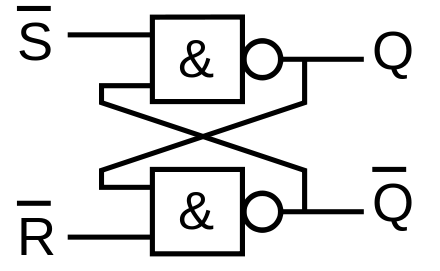
\includegraphics[width=0.60\linewidth]{images/processeurs_porte_bascule_nand.png}
        \caption{Implémentation à partir de portes \textit{NON-ET}}
        \label{pic_processeurs_porte_bascule_nand}
    \end{subfigure}
    ~ %add desired spacing between images, e. g. ~, \quad, \qquad, \hfill etc. 
      %(or a blank line to force the subfigure onto a new line)
    \begin{subfigure}[]{0.48\linewidth}\centering
        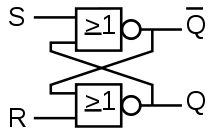
\includegraphics[width=0.60\linewidth]{images/processeurs_porte_bascule_nor.png}
        \caption{Implémentation à partir de portes \textit{NON-OU}}
        \label{pic_processeurs_porte_bascule_nor}
    \end{subfigure}
    \caption{Réalisation d'une bascule à partir de deux types de portes. La bascule maintient son état actuelle tant que les signaux d'entrée ne changent pas}
    \label{fig_processeurs_porte_bascule}
\end{figure}


\subsection{Les mémoires RAM} \label{sec:ram}
%%%%%%%%%%%%%%%%%%%%%%%%%%%%%%%%%%%%%%%%%%%%%%%%%%%%%%%%%%%%%%%%%%%

La mémoire à accès aléatoires ou \textit{Random Acces Memory} (RAM) est une mémoire dont le temps d'accès ne dépend pas de la position de l'information. Contrairement aux disques ou aux bandes magnétiques dont le temps d'accès pouvait varier en fonction de l'emplacement actuel de la tête de lecture et de la prochaine donnée à lire. La RAM est une mémoire volatile, l'information stockée n'est pas persistante lorsque la mémoire n'est plus alimentée. Il y a eu beaucoup d'évolution des différentes technologies RAM depuis leur création. Il en existe différents types, ayant leurs avantages et leurs inconvénients. Dans une plate-forme actuelle, deux types de mémoires RAM sont principalement utilisées: la RAM statique (SRAM, \autoref{pic_processeurs_porte_sram}) et la RAM dynamique (DRAM, \autoref{pic_processeurs_porte_sram}). La raison principale de la présence de deux types de RAM vient de leur différence de coût de production. La SRAM, bien que plus rapide, est aussi beaucoup plus chère. Cette différence de prix s'explique par l'architecture des deux mémoires ((\autoref{fig_processeurs_ram}).


\begin{figure}
    %\centering
    \begin{subfigure}[]{0.48\linewidth}\centering
        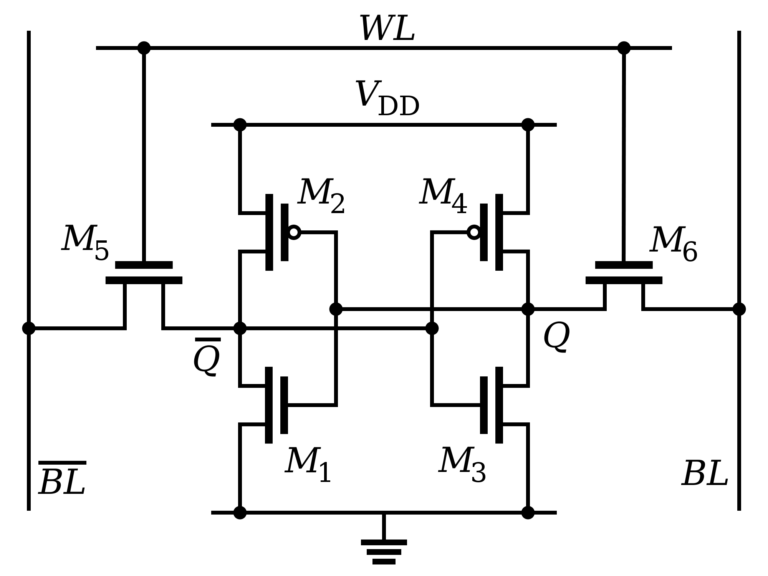
\includegraphics[width=0.60\linewidth]{images/processeurs_porte_sram.png}
        \caption{Mémoire vive statique (SRAM) utilisant 6 transistors}
        \label{pic_processeurs_porte_sram}
    \end{subfigure}
    ~ %add desired spacing between images, e. g. ~, \quad, \qquad, \hfill etc. 
      %(or a blank line to force the subfigure onto a new line)
    \begin{subfigure}[]{0.48\linewidth}\centering
        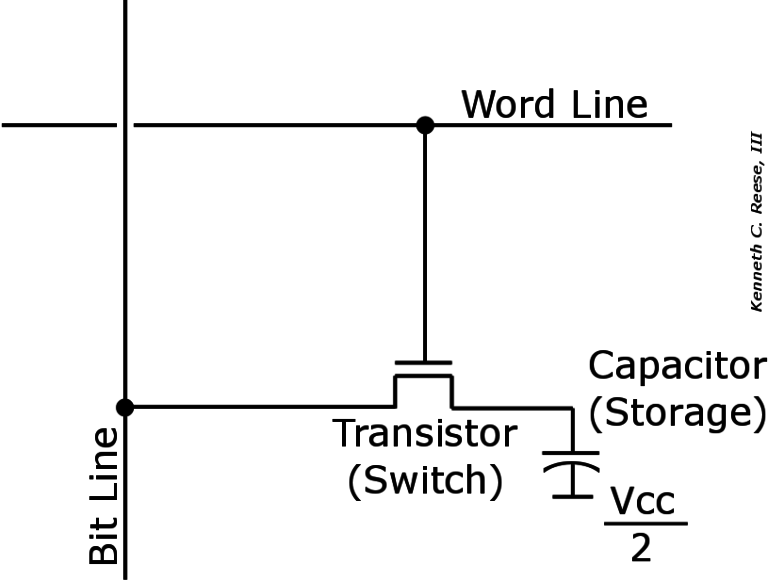
\includegraphics[width=0.60\linewidth]{images/processeurs_porte_dram.png}
        \caption{Mémoire vive dynamique (DRAM) utilisant un condensateur et un transistor}
        \label{pic_processeurs_porte_sram}
    \end{subfigure}
    \caption{Deux types de RAM très utilisées dans les architectures. La différence de complexité de leur circuit électronique explique la différence de prix entre les deux technologies}
    \label{fig_processeurs_ram}
\end{figure}

\subsubsection{La SRAM} 
La RAM statique est un circuit logique qui utilise 6 transistors pour représenter les états 0 et 1 (bien qu'il existe des variantes utilisant 4, 8 ou même 10 transistors). Une SRAM à 6 transistors en utilise 4 pour stocker l'information. Deux transistors additionnels sont utilisés pour contrôler leur accès durant leur lecture ou écriture.
Il est courant d'utiliser différents types de SRAM dans les différents niveaux de caches pour optimiser la densité (mémoire de plus grande capacité) ou la vitesse d'accès. Le premier niveau de cache étant optimisé pour la vitesse d'accès, contrairement aux caches de niveau supérieur de plus grande capacité.


\subsubsection{La DRAM} 
La RAM dynamique a une structure plus simple que la SRAM qui n'est composée que d'un transistor et d'un condensateur. La valeur du bit est déterminée par la charge (positive ou négative) du condensateur. Qu'il soit VRAI ou FAUX, le condensateur doit donc être chargé. 
À cause des fuites (\textit{leakage}) les condensateurs doivent être rafraîchis en permanence. La fréquence de rafraîchissement est de l'ordre de 1\% à 5\% du temps total d'utilisation de la mémoire. C’est cette spécificité qui fait de la DRAM une mémoire très consommatrice en énergie. Grâce à leur faible nombre de transistors, la densité des mémoires DRAM est élevée permettant la construction de mémoire de grande capacité (en GiB). Cependant, la lecture d’une cellule décharge le condensateur, il faut donc, même lors d’une lecture, le recharger.
La charge et la décharge du condensateur n’étant pas instantanés, la DRAM est beaucoup plus lente que la SRAM (une cellule ne pouvant pas être accédée pendant son rafraîchissement).
La quasi-totalité des ordinateurs des 50 dernières années ont une mémoire centrale utilisant de la DRAM.

%Il existe plusieurs types de DRAM: DDR, GDDR, QDR, HBMC, HMC.


\subsubsection{SRAM vs DRAM}

L'avantage de la SRAM est sa rapidité de fonctionnement et sa faible consommation électrique. Contrairement à la DRAM, la SRAM est statique, elle conserve l'information et ne nécessite pas de rafraîchissement périodique pour conserver la donnée enregistrée. Cependant, elle s'efface si aucune tension ne lui est appliquée en continu.
Le principal inconvénient de la SRAM vient de son coût de fabrication ainsi que leur faible densité (due à l'utilisation de 6 transistors)


\begin{table}[]
\begin{tabular}{l|l|l|}
\cline{2-3}
                                       & SRAM     & DRAM             \\ \hline
\multicolumn{1}{|l|}{Prix/bit}         & élevé    & bas              \\ \hline
\multicolumn{1}{|l|}{Vitesse d'accès}  & rapide   & lent             \\ \hline
\multicolumn{1}{|l|}{Latence}          & 0.5-5 ns & 50-70 ns        \\ \hline
\multicolumn{1}{|l|}{Rafraichissement} & non      & oui              \\ \hline
\multicolumn{1}{|l|}{Consommation}     & basse    & élevée           \\ \hline
\multicolumn{1}{|l|}{Énergie/bit}      & n pj     & n pj             \\ \hline
\multicolumn{1}{|l|}{Densité}          & faible (6 transistors par bit)   & élevée (1 transistor par bit)          \\ \hline
\multicolumn{1}{|l|}{Complexité}       & grande   & faible           \\ \hline
\multicolumn{1}{|l|}{Utilisation}      & Cache    & Mémoire centrale \\ \hline
\multicolumn{1}{|l|}{Endurance}        & todo     & $10^{16}$           \\ \hline
\end{tabular}
\end{table}




\subsection{Évolution des transistors}
%%%%%%%%%%%%%%%%%%%%%%%%%%%%%%%%%%%%%%%%%%%%%%%%%%%%%%%%%%%%%%%%%%%


La vitesse de calcul d'un processeur ou la capacité de stockage d'une mémoire sont directement liées au nombre de transistors disponible sur une puce. 
Plus un processeur aura de transistors, au plus il pourra calculer rapidement (ajout de coeur, meilleures unités de calculs). Plus une mémoire aura de transistors, au plus elle pourra contenir de cellule RAM et donc avoir une grande capacité de stockage. La performance des systèmes informatiques est donc directement liée aux technologies de transistors utilisées. 


\subsubsection{Évolution du nombre de transistors.} \label{sec:moore}

L'évolution du nombre de transistors sur une puce a été prédite par l'un des trois fondateurs de la société Intel, Gordon Moore. En 1965, Gordon Moore prévoit que le nombre de transistors d'un puce doublera chaque année, sur une même surface et pour un coût constant \cite{Moore1998}. Il réévaluera cette période à 2 ans en 1975 \cite{Moore75}, ce qui correspond parfaitement avec l'évolution réelle jusqu'à ces dernières années (\autoref{pic_Moore_prediction}).




\begin{figure}
    %\centering
    \begin{subfigure}[]{0.48\linewidth}\centering
        \vspace{1cm}
        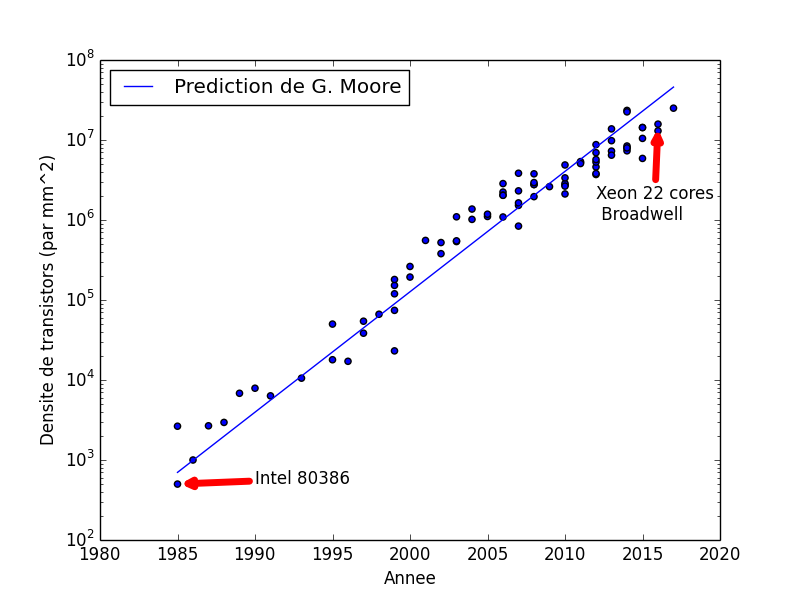
\includegraphics[width=\linewidth]{images/Chapitre1/Moore_prediction.png}
        \caption{\label{pic_Moore_prediction} Évolution du nombre de transistors des processeurs Intel (données \cite{Wikipedia2019Transistor})}
    \end{subfigure}
    ~ %add desired spacing between images, e. g. ~, \quad, \qquad, \hfill etc. 
      %(or a blank line to force the subfigure onto a new line)
    \begin{subfigure}[]{0.48\linewidth}\centering
        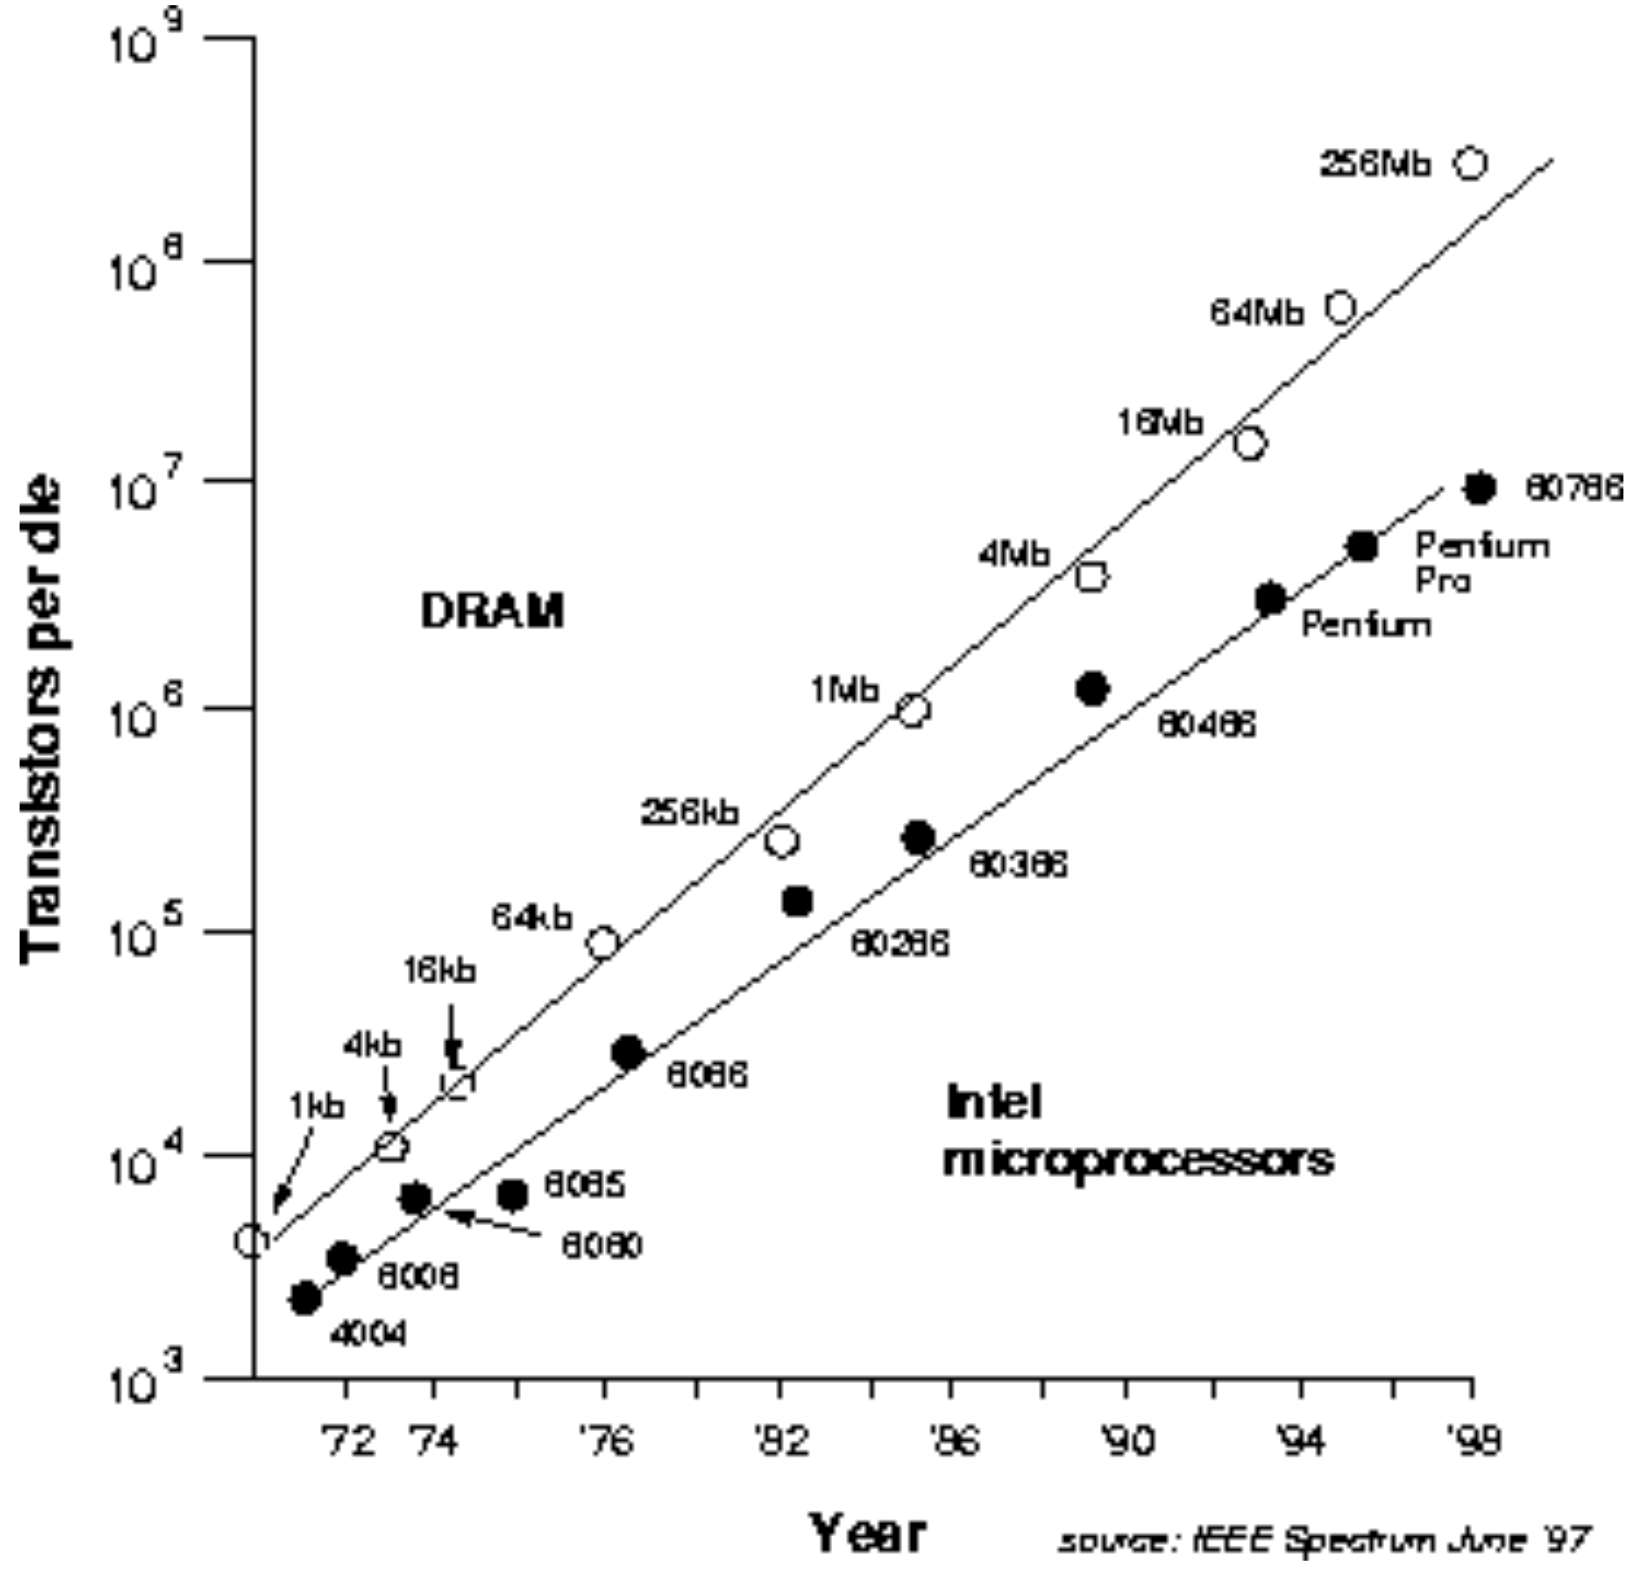
\includegraphics[width=0.9\linewidth]{images/processeurs_porte_moore_dram.png}
        \caption{La loi de Moore s'applique aux processeurs comme aux mémoires DRAM.}
        \label{processeurs_porte_moore_dram}
    \end{subfigure}
    \caption{La loi de Moore décrit l'évolution de la densité de transistors qui double tous les deux ans pour un prix constant.}
    \label{fig_processeurs_moore}
\end{figure}





\subsubsection{Coût de la gravure.}

Depuis plus de cinquante ans, les \textbf{fondeurs} (les industriels responsables de la gravure des processeurs) tels que Samsung Electronics, TSMC, Intel et GlobalFoundries ont développé de nombreuses techniques et technologies pour réduire la taille des transistors (voir \autoref{processeurs_porte_fondeurs}). Aujourd'hui, de nombreuses étapes sont nécessaires pour transformer une plaque de silicium (la plus pure possible) en processeurs: dopage, déposition d'une couche de résine, gravure, traitement thermique, revêtement par couche mince, découpe, encapsulation... \cite{AnthonyNelzinSantos2018}.

Les procédés de fabrication étant plus complexes, les usines de fabrication coûtent elles aussi de plus en plus cher. L'augmentation du coût des fonderies a elle aussi été prédite par la seconde loi de Gordon Moore (ou \textit{loi de Rock}), qui estime que leur prix double tous les 4 ans \cite{schaller1997moore}. Bien que les coûts de fabrication augmentent, la taille de gravure s’affine et permet de mettre plus de transistors sur une même surface, permettant ainsi à l’industrie de suivre la cadence dictée par la loi de Moore (\autoref{pic_Moore_explique}).

Cependant, les finesses de gravures utilisées aujourd'hui sont tellement faibles qu'elles atteignent une limite physique, celle de la taille des atomes. À des tailles proches de quelques atomes, les courants électriques ne sont plus stables et la course à la réduction des finesses de gravure n'a jamais été aussi difficile. Voilà plusieurs années, qu'Intel ne parvient plus à descendre sous les 10 nm. Les procédés à mettre en oeuvre pour y parvenir sont si complexes, qu'il est courant de parler de la fin de la loi de Moore \cite{theis2017end}. En 2019, Samsung annonce qu'il a mis au point une technologie permettant la gravure des premiers processeurs en 3 nm dès 2021 \cite{AdrianBRANCO2019}. 


\begin{figure}[htbp]
    \centering
    \begin{subfigure}[b]{0.40\linewidth}\centering
        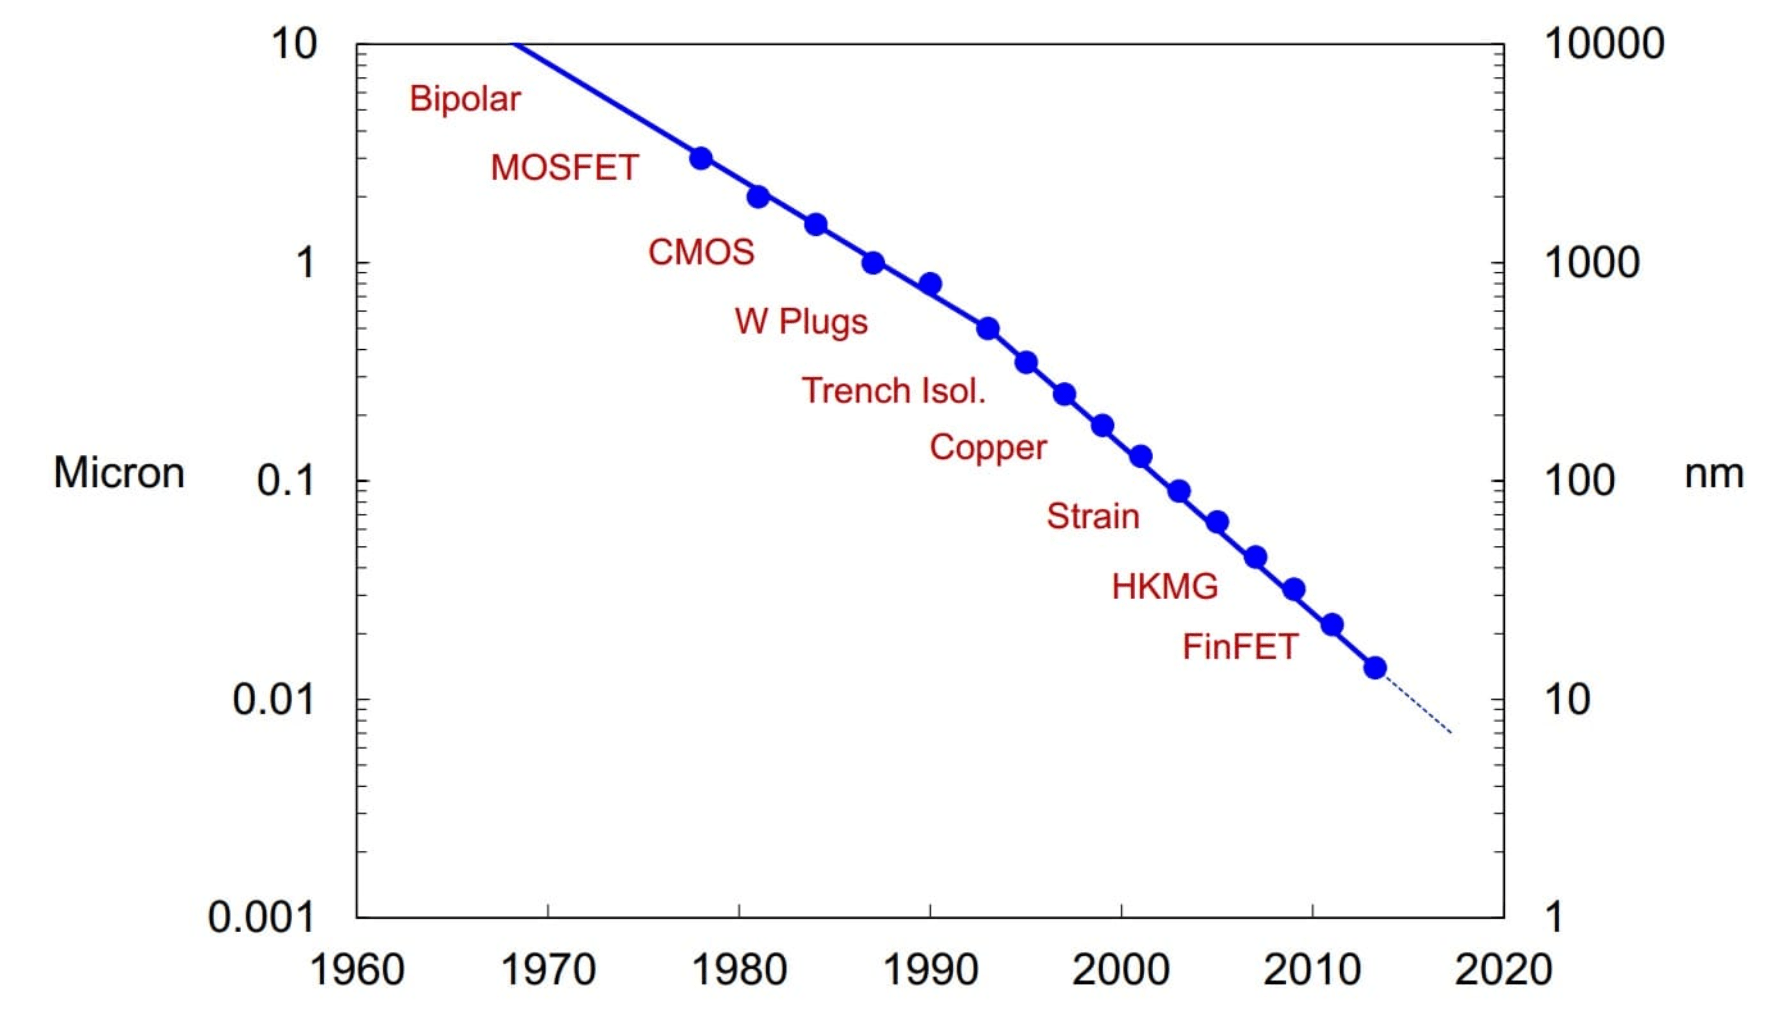
\includegraphics[width=\linewidth]{images/processeurs_porte_fondeurs.png}
        \caption{\label{processeurs_porte_fondeurs} Les technologies utilisées pour la gravure ont évoluées, rendant les fonderies plus performantes mais aussi plus chères (source Intel).}.
    \end{subfigure}
    ~ %add desired spacing between images, e. g. ~, \quad, \qquad, \hfill etc.
      %(or a blank line to force the subfigure onto a new line)
    \begin{subfigure}[b]{0.50\linewidth}\centering
        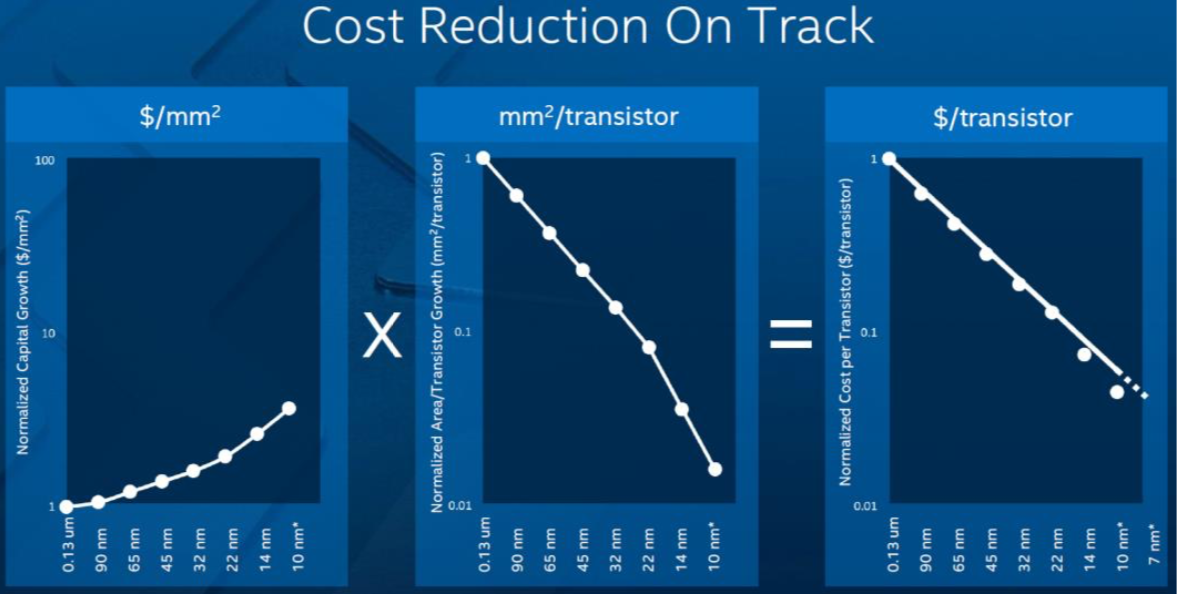
\includegraphics[width=\linewidth]{images/processeurs_porte_moore.png}
        \caption{\label{pic_Moore_explique} Bien que le prix des fonderie augmente, le nombre de transistors gravable sur une puce augmente plus rapidement. Conséquence de la loi de Moore: le prix par transistor diminue exponentiellement.}
    \end{subfigure}
    \caption{Les nouvelles technologies utilisées dans les fonderies permettent de graver des transistors toujours plus petits.}\label{pic_fonderie}
\end{figure}









%%%%%%%%%%%%%%%%%%%%%%%%%%%%%%%%%%%%%%%%%%%%%%%%%%%%%%%%%%%%%%%%%%%
%%%%%%%%%%%%%%%%%%%%%%%%%%%%%%%%%%%%%%%%%%%%%%%%%%%%%%%%%%%%%%%%%%%

